\documentclass[10pt,a4paper]{article}

\usepackage[a4paper,margin=18mm,top=16mm,bottom=16mm]{geometry}
\usepackage[T1]{fontenc}
\usepackage[utf8]{inputenc}
\usepackage{lmodern}
\usepackage{microtype}
\usepackage{graphicx}
\usepackage{xcolor}
\usepackage{tikz}
\usetikzlibrary{arrows.meta,positioning,calc}
\usepackage{tabularx}
\usepackage{array}
\usepackage{enumitem}
\usepackage{booktabs}
\usepackage{hyperref}
\usepackage{titlesec}
\usepackage{fancyhdr}
\usepackage{parskip}

\definecolor{Ink}{HTML}{151515}
\definecolor{Muted}{HTML}{6B6B6B}
\definecolor{Rule}{HTML}{D8D8D8}
\definecolor{Soft}{HTML}{F5F5F3}
\definecolor{Soft2}{HTML}{FAFAF8}

\hypersetup{
  colorlinks=true,
  urlcolor=Ink,
  linkcolor=Ink,
  pdftitle={Project Proposal - Pedestrian Flow Forecasting},
  pdfauthor={Timo Schlumpf}
}

\setlength{\parindent}{0pt}
\setlength{\parskip}{4.5pt}
\setlist[itemize]{leftmargin=1.3em,itemsep=1pt,topsep=2pt}

\titleformat{\section}
  {\large\bfseries\color{Ink}}
  {\thesection}{0.5em}{}
  [\vspace{1pt}\titlerule]
\titlespacing*{\section}{0pt}{7pt}{4pt}

\pagestyle{fancy}
\fancyhf{}
\renewcommand{\headrulewidth}{0pt}
\fancyfoot[L]{\scriptsize\color{Muted}MLOps HS26}
\fancyfoot[R]{\scriptsize\color{Muted}Project Proposal \textbullet{} \thepage}

\newcommand{\ProjectTitle}{Predicting Pedestrian Flow}
\newcommand{\Subtitle}{A 60-minute forecasting system for urban footfall}
\newcommand{\MetaLabel}[1]{\textsc{\scriptsize\color{Muted}#1}}

\begin{document}

% ===================== PAGE 1 =====================
\thispagestyle{empty}

\noindent
\begin{minipage}[t]{0.22\textwidth}
  \vspace{0pt}
\includegraphics[width=16mm]{logo.pdf}
\end{minipage}%
\hfill
\begin{minipage}[t]{0.70\textwidth}
  \vspace{0pt}\raggedleft\scriptsize\color{Muted}MLOps \textbullet{} HS26 \textbullet{} Project Proposal \textbullet{} Machine Learning Operations \textbullet{} HSLU
\end{minipage}
\vspace{2.8mm}
{\fontsize{22}{26}\selectfont\bfseries\ProjectTitle\par}
\vspace{1.2mm}
{\fontsize{13.5}{17}\selectfont\color{Muted}\Subtitle\par}

\vspace{7mm}
\color{Ink}\rule{\textwidth}{0.8pt}
\vspace{4mm}

{\small\color{Muted}
A live machine-learning system that forecasts pedestrian traffic at a monitored urban location one hour into the future, using public mobility, weather and temporal context.\par}

\vspace{12mm}

\renewcommand{\arraystretch}{1.45}
\begin{tabularx}{\textwidth}{@{}>{\raggedright\arraybackslash}p{18mm}X@{}}
\MetaLabel{WHO} & Businesses operating in high-footfall areas: shops, restaurants and other local operators that benefit from anticipating near-term demand. The system is designed around public data, with private customer-count integration left as a future extension.\\
\MetaLabel{WHERE} & Z\"urich, Switzerland. The initial target is the Hystreet counter at Lintheschergasse, with public-transport activity around Z\"urich HB as future context.\\
\MetaLabel{WHEN} & Primary prediction horizon: the next 60-minute interval. The inference system runs on a schedule; the same forecasting step can be run recursively to produce longer-range forecasts, with uncertainty compounding across steps.\\
\MetaLabel{WHAT} & Predict the number of pedestrians recorded during the next hour. The target is pedestrian flow, not an estimate of shoppers, commuters or people physically present at an instant.\\
\MetaLabel{WHY} & Near-term footfall is an operational signal. A reliable forecast can support staffing, preparation, stock decisions and other time-sensitive planning while remaining based on data a small business could plausibly access.\\
\end{tabularx}

\vspace{10mm}

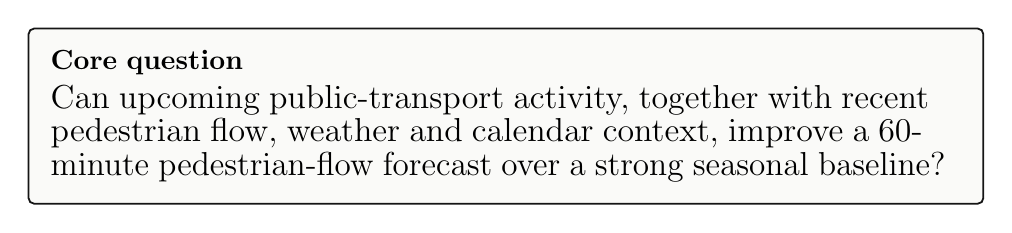
\begin{tikzpicture}
  \node[draw=Ink, line width=0.65pt, rounded corners=2pt, fill=Soft2, inner sep=8pt, text width=\dimexpr\textwidth-16pt\relax] {
    \textbf{Core question}\par\vspace{2pt}
    \large Can upcoming public-transport activity, together with recent pedestrian flow, weather and calendar context, improve a 60-minute pedestrian-flow forecast over a strong seasonal baseline?
  };
\end{tikzpicture}

\vfill

{\scriptsize
\begin{tabularx}{\textwidth}{@{}X X@{}}
\textbf{Author} & \textbf{Repository}\\
Timo Schlumpf & \href{https://github.com/0xff4b/gaeja}{github.com/0xff4b/gaeja}\\
\end{tabularx}
}

\vspace{3mm}
{\scriptsize\color{Muted}Prepared 01 October 2026 \textbullet{} Autumn Semester 2026}

\newpage

% ===================== PAGE 2 =====================
\fontsize{8.9}{10.15}\selectfont
\setlength{\parskip}{2.2pt}
\titlespacing*{\section}{0pt}{3.5pt}{2pt}

\section{Problem statement}
Businesses in high-footfall areas can benefit from knowing how busy their surroundings will be before the next hour begins. This project predicts the \textbf{total number of pedestrians recorded at a monitored location during the next 60-minute interval}, using only information available at prediction time.

The initial target will be the Hystreet measurement area at Lintheschergasse in Z\"urich, with the other Hystreet areas used as spatial context. The City of Z\"urich publishes measurements supplied by hystreet.com GmbH; they are updated hourly and provide more than five years of historical coverage, with the dataset continuing to grow by new hourly observations. The primary success criterion is a \textbf{relative 10\% reduction in MAE versus a seasonal-naive baseline}: MAE must be at most 90\% of the baseline MAE. The seasonal-naive forecast is the observed count from the same location one week earlier (t-168 hours). The 10\% margin is intended as a meaningful but deliberately modest improvement threshold: it requires a measurable gain over a strong temporal baseline without imposing an arbitrary absolute error target. Persistence will be reported as a second baseline. Evaluation will use an out-of-time test period.

\section{Originality \& motivation}
The intended product is a forecasting service for shops, restaurants and other businesses where pedestrian traffic affects staffing, preparation, stock and operations. It deliberately forecasts an observable quantity: counted pedestrians are not assumed to be customers. A future store integration could calibrate public footfall against private customer-count data. The project also builds on an existing weather-data ingestion prototype, making the initial data-engineering scope realistic while leaving the ML and MLOps layers as the core work.

The central modelling idea is to treat \textbf{upcoming public-transport services as future-known structured context}. Instead of using only a scalar ``trains next hour'' feature, the model receives the scheduled events in the prediction horizon, including their timing and service characteristics. The project therefore asks whether the composition of future mobility improves short-horizon pedestrian forecasting beyond historical flow, weather and calendar context. This differentiates the project from generic traffic forecasting. The concept was checked against previous HSLU and KTH ID2223 project topics.

\section{Data source \& features}
\begin{center}
\fontsize{8.1}{9.1}\selectfont
\renewcommand{\arraystretch}{1.06}
\begin{tabular}{@{}>{\bfseries}p{28mm}p{55mm}p{42mm}@{}}
\toprule
Source & Used for & Notes \\
\midrule
Hystreet / Z\"urich Open Data & Target; lags 1, 2, 3, 6, 24, 168 h; rolling means 3, 6, 24, 168 h; spatial context & Public CSV/Parquet dataset supplied by hystreet.com GmbH; updated hourly; no scraping; historical + ongoing. \\
Z\"urich weather & Temperature, precipitation, humidity, pressure, wind & REST API + historical downloads; only values available at prediction time are used. \\
Swiss GTFS & Upcoming public-transport events & Dated timetable snapshots; each event encoded by time-to-arrival/departure, service type and line. \\
Z\"urich school holidays & Hour, weekday, weekend, public holiday, school holiday & Deterministic calendar features. \\
\bottomrule
\end{tabular}
\end{center}

The label is the observed pedestrian count in the future hourly interval and is not mechanically derived from the inputs. This is a continuous regression target; rare-positive-class handling is not applicable. Backfill uses only information available at each historical prediction timestamp. For GTFS, the latest archived timetable snapshot available on or before the timestamp is used when its validity covers the prediction horizon; later revisions are excluded. Future pedestrian observations, future weather and final train outcomes are never inputs. Missing sensor intervals are handled from timestamps rather than row position. GTFS-RT delays and train-occupancy forecasts remain optional extensions.

\section{System design}
The project follows the required Feature--Training--Inference (FTI) architecture. The core system prioritizes reliable ingestion, backfill, feature storage, reproducible training and serving.

\begin{center}
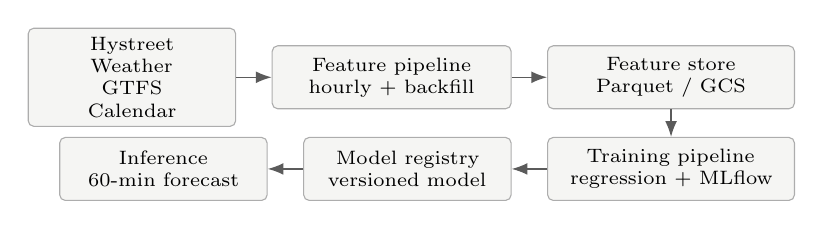
\begin{tikzpicture}[
  node distance=3.5mm and 4.5mm,
  box/.style={draw=Ink!35, rounded corners=2pt, fill=Soft, minimum height=8mm, text width=24mm, align=center, font=\scriptsize},
  arrow/.style={-{Latex[length=2mm]}, line width=0.5pt, draw=Ink!70}
]
  \node[box] (data) {Hystreet\\Weather\\GTFS\\Calendar};
  \node[box, right=of data, text width=28mm] (feat) {Feature pipeline\\hourly + backfill};
  \node[box, right=of feat, text width=29mm] (store) {Feature store\\Parquet / GCS};
  \node[box, below=of store, text width=29mm] (train) {Training pipeline\\regression + MLflow};
  \node[box, left=of train, text width=24mm] (reg) {Model registry\\versioned model};
  \node[box, left=of reg, text width=24mm] (inf) {Inference\\60-min forecast};
  \draw[arrow] (data) -- (feat);
  \draw[arrow] (feat) -- (store);
  \draw[arrow] (store) -- (train);
  \draw[arrow] (train) -- (reg);
  \draw[arrow] (reg) -- (inf);
\end{tikzpicture}
\end{center}

The feature pipeline runs on a schedule and supports historical backfill. The training pipeline retrains on matured labels, evaluates against the baselines, tracks experiments with MLflow and registers the selected model. The inference pipeline joins the current feature state with retrieved upcoming transport events and serves the next-hour forecast through a lightweight web UI. Once the interval has elapsed, the observed footfall count becomes a matured label for a later training run.

\begin{center}
\scriptsize
\begin{tabular}{@{}>{\bfseries}p{27mm}p{91mm}@{}}
\toprule
Python & ingestion, feature computation and model code \\
Docker & reproducible pipelines and inference \\
GitHub Actions & scheduled pipelines and CI \\
Parquet / GCS & versioned feature storage and backfill \\
MLflow & experiment tracking and model registry \\
FastAPI + web dashboard & prediction serving and live model output \\
\bottomrule
\end{tabular}
\end{center}

Feature definitions will be shared between training and inference. The repository is public and kept reachable throughout the semester. Optional extensions include GTFS-RT disruptions, train-occupancy context, richer event data and additional monitoring; the core FTI system is built first.



\end{document}
